\section{Reconhecimento dos Usuários}
	 
	O reconhecimento facial do Sistema TRUE foi implementado utilizando imagens de cor como dados de entrada. Portanto, ele tem influência de diversos fatores como iluminação, ângulo, pose, expressões, cosméticos e acessórios. Para análise dos resultados foi utilizada como ferramenta uma matriz de confusão construída a partir dos dados coletados do sistema. Matriz de confusão consiste em uma matriz onde as colunas representam os possíveis valores que se podem obter para cada usuário e as linhas os usuários que foram observados. Os valores presentes na matriz representam os resultados em porcentagens de testes de reconhecimento realizados com alguns usuários. Então, a matriz permite a fácil visualização da confiança obtida no reconhecimento observando-se os valores obtidos na diagonal principal que representam as porcentagens de acerto para cada usuário.

	Para se ter uma melhor interpretação dos valores presentes na matriz de confusão, as três taxas a seguir poderm ser obtidas a partir da matriz:

	\begin{enumerate}
		\item \textbf{Verdadeiro Positivo}: quando o sistema identifica o usuário de maneira correta.
		\item \textbf{Verdadeiro Negativo}: quando o sistema identifica o usuário de maneira errada.
		\item \textbf{Falso Negativo}: quando o sistema não identifica o usuário cadastrado.
	\end{enumerate}

	Foram realizados dois conjuntos de testes para avaliar a precisão do reconhecimento facial implementado no Sistema TRUE. Os cenários desses testes foram compostos por usuários previamente cadastrados, além das 40 pessoas cadastradas no banco de faces da Universidade de Cambridge~\cite{cambridgeFaceDb}. No primeiro conjunto de testes foram previamente cadastrados 11 usuários e no segundo 10 usuários. Nesses testes, cada usuário se posicionou em frente ao \textit{Kinect}, com o rosto na posição frontal em relação ao sensor. Com isso, o sistema realizou o processo de reconhecimento facial 20 vezes para cada usuário. Os dois conjuntos de testes foram necessários tendo em vista que os resultados do primeiro não foram satisfatórios. A diferença entre ambos está na estratégia utilizada no cadastro dos usuários no sistema. 

		\begin{figure}[htb]
			\begin{center}
				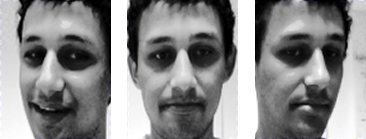
\includegraphics[scale=0.4]{figuras/4.ProblemaEProposta/face-registro.png}
			\end{center}
			\caption{Exemplo de imagens obtidas na etapa de cadastro do usuário.}
			\label{fig:imgs-cadastro}
		\end{figure}	

	No primeiro conjunto de testes, os cadastrados dos usuários foram feitos utilizando 10 imagens de faces de cada usuário: 6 imagens frontais da face, 2 imagens da face ligeiramente rotacionada para direita e 2 imagens da face ligeiramente rotacionada para esquerda. A Figura~\ref{fig:imgs-cadastro} exemplifica imagens de face obtidas nestes cadastros. Os cadatros foram realizados com essa estratégia com o objetivo de diminuir o impacto das variações de poses e ângulo no reconhecimento facial. Os resultados obtidos dos processos de reconhecimento facial realizados para cada usuário são mostrados na matriz de confusão representada pela Tabela~\ref{tab:matriz-confusao}. 

	\begin{table}[htb]
		\begin{center}
			\caption{Matriz de confusão para apresentar os resultados obtidos no primeiro conjunto de testes.}
			\label{tab:matriz-confusao}
			\begin{tabular}{|c|c|c|c|c|c|c|c|c|c|c|c|c|}
				\hline  & \bf \begin{sideways}Tales\end{sideways} & \bf \begin{sideways}Danilo\end{sideways} & \bf \begin{sideways}Ana\end{sideways} & \bf \begin{sideways}Fabricio\end{sideways} & \bf \begin{sideways}Lucas\end{sideways} & \bf \begin{sideways}Bruno\end{sideways} & \bf \begin{sideways}Ricardo\end{sideways} & \bf \begin{sideways}Estevao\end{sideways} & \bf \begin{sideways}Rafael\end{sideways} &
				\bf \begin{sideways}Vinicius\end{sideways} & \bf \begin{sideways}Pedro\end{sideways} & \bf \begin{sideways}Desconhecido\end{sideways}\\ 
				
				\hline \bf Tales 		& 95\% & 			& 		 & 			&   	 & 			& 		 & 			& 		 & 			& 		 & 5\%	\\ 
				\hline \bf Danilo 	& 		 & 75\% & 		 & 			&   	 & 			& 		 & 			& 		 & 			& 25\% &		 	\\
				\hline \bf Ana 			& 		 & 			& 95\% & 			&   	 & 			& 		 & 			& 		 & 			& 		 & 5\%  \\
				\hline \bf Fabricio & 20\% & 			& 		 & 50\% &      & 			& 10\% & 			&  	   & 20\% & 		 &		  \\
				\hline \bf Lucas 		& 		 & 			& 		 & 			& 55\% & 			& 		 & 			& 		 & 			& 20\% & 25\% \\
				\hline \bf Bruno 		& 5\%	 & 			& 		 & 			& 		 & 70\% & 		 & 			& 10\% & 	5\%	& 		 & 10\%	\\
				\hline \bf Ricardo 	& 		 & 			& 10\% & 			& 		 & 			& 85\% & 			& 		 & 			& 		 & 5\%  \\
				\hline \bf Estevao 	& 		 & 			& 		 & 			& 		 & 			& 		 & 70\% & 		 & 			& 		 & 30\% \\
				\hline \bf Rafael 	& 10\% & 	5\%	& 		 & 			& 10\% & 			& 		 & 			& 45\% & 20\% & 		 & 10\% \\
				\hline \bf Vinicius & 		 & 			& 5\%  & 			& 		 & 			& 		 & 			& 5\%  & 70\% & 10\% & 10\% \\
				\hline \bf Pedro 		& 		 & 			& 		 & 			& 		 & 			& 		 & 			& 		 & 			& 100\%&		  \\
				\hline
			\end{tabular}
		\end{center}
	\end{table}

	Como previsto, pode-se observar na matriz que os maiores valores estão na diagonal principal. Alguns resultados obtidos foram satisfatórios com porcentagens maiores que 90\%. Por outro lado, foram obtidos alguns resultados com baixas porcentagens como 45\%. Estes últimos foram principalmente causados por problemas como pose e expressões faciais. A iluminação não foi um problema, pois no ambiente de teste não existe influência da iluminação externa e a interna é controlada. 

	Tais taxas foram inseridas na Tabela~\ref{tab:taxas}. A taxa de acerto
	(verdadeito positivo) foi menor do que se esperava. Portanto, o teste foi
	realizado novamente utilizando menos usuários, 6 usuários além dos 40
	presentes no banco de faces da Universidade de
	Cambridge~\cite{cambridgeFaceDb}. Porém o cadastro destes usuários foi feito
	de maneira diferente. Ao invés de se obter 10 fotos das faces posicionadas de
	maneira frontal em relação ao sensor, foram obtidas 100 imagens das faces em
	diferentes ângulos, posições e expressões faciais. Os resultados obtidos, foram inseridos em uma
	segunda matriz de confusão (Tabela~\ref{tab:matriz-confusao2}).

	\begin{table}[htb]
		\begin{center}
			\caption{Taxas obtidas para o primeiro conjunto de testes de identificação.}
			\label{tab:taxas}
			\begin{tabular}{|l|c|}
				\hline \bf Verdadeiro Positivo & 73,63\% \\
				\hline \bf Verdadeiro Negativo & 17,27\% \\
				\hline \bf Falso Negativo & 9,10\% \\
				\hline
			\end{tabular}
		\end{center}
	\end{table}


	% \begin{table}[htb]
	% 	\begin{center}
	% 		\caption{Matriz de confusão para apresentar os resultados obtidos.}
	% 		\label{tab:matriz-confusao2}
	% 		  \begin{tabular}{|c|c|c|c|c|c|c|c|c|}
	% 			% \hline  & \bf \ref{user:tales} & \bf \ref{user:danilo} & \bf
	% 			% \ref{user:ana} & \bf \ref{user:fabricio} & \bf \ref{user:lucas} & \bf
	% 			% \ref{user:bruno} &  \bf Desconhecido\\

	% 			\hline  & \bf Tales & \bf Danilo & \bf Ana & \bf Fabricio & \bf Lucas & \bf Bruno &  \bf Desconhecido\\
				 
	% 			\hline \bf Tales 		& 90\% & 			& 		 & 			&   	 & 			& 10\%		\\
	% 			\hline \bf Danilo 	& 		 & 100\%& 		 & 			&   	 & 			& 		 		\\
	% 			\hline \bf Ana 			& 		 & 			& 100\%& 			&   	 & 			& 		    \\
	% 			\hline \bf Fabricio & 		 & 			& 		 &100\%      &      & 			&      		\\
	% 			\hline \bf Lucas 		& 		 & 			& 		 & 			& 85\% & 			& 15\%		\\
	% 			\hline \bf Bruno 		& 		 & 			& 		 & 			& 		 & 100\%& 		  	\\
	% 			\hline
	% 		\end{tabular}
	% 	\end{center}
	% \end{table}

	\begin{table}[htb]
		\begin{center}
			\caption{Matriz de confusão para apresentar os resultados obtidos no segundo conjunto de testes.}
			\label{tab:matriz-confusao2}
			  \begin{tabular}{|c|c|c|c|c|c|c|c|c|c|c|c|c|}
				% \hline  & \bf \ref{user:tales} & \bf \ref{user:danilo} & \bf
				% \ref{user:ana} & \bf \ref{user:fabricio} & \bf \ref{user:lucas} & \bf
				% \ref{user:bruno} &  \bf Desconhecido\\

				\hline  & \bf \begin{sideways}Tales\end{sideways} & \bf \begin{sideways}Danilo\end{sideways} & \bf \begin{sideways}Ana\end{sideways} & \bf \begin{sideways}Fabricio\end{sideways} & \bf \begin{sideways}Lucas\end{sideways} & \bf \begin{sideways}Bruno\end{sideways} & \bf \begin{sideways}Carla\end{sideways} & \bf \begin{sideways}Marcela\end{sideways} & \bf \begin{sideways}Caio\end{sideways} & \bf \begin{sideways}Marcelo\end{sideways} & \bf \begin{sideways}Desconhecido\end{sideways}\\
				 
				\hline \bf Tales 			&100\% & 			& 		 & 			&   	 & 			& 		& 		&	 		& 		& 		\\
				\hline \bf Danilo 		& 		 &100\%	& 		 & 			&   	 & 			& 		& 		& 		& 		& 		 		\\
				\hline \bf Ana 				& 		 & 			& 		 & 			&   	 & 			& 		& 		& 		& 		& 		    \\
				\hline \bf Fabricio 	& 		 & 			& 		 &45\%	&      & 			& 		& 		& 		& 5\%	& 50\%    		\\
				\hline \bf Lucas 			& 		 & 			& 		 & 			& 85\% & 			& 		& 		& 		& 		& 15\%		\\
				\hline \bf Bruno 			& 		 & 			& 		 & 			& 		 & 75\% & 	  & 		&20\% & 5\%	& 		  	\\
				\hline \bf Carla 			& 		 & 			& 		 & 			& 		 & 			&85\% &		  & 	  & 		& 15\%		  	\\
				\hline \bf Marcela 		& 		 & 			& 		 & 			& 		 &      & 		&65\% &10\% & 		& 25\%		  	\\
				\hline \bf Caio 		  & 		 & 			& 		 & 			& 	5\%& 	15\%& 		& 		&80\%	&	 		& 		  	\\
				\hline \bf Marcelo 		& 		 & 			& 		 & 			& 		 & 			& 		& 		& 		& 90\%& 10\%		  	\\
				\hline
			\end{tabular}
		\end{center}
	\end{table}

	\begin{table}[htb]
		\begin{center}
			\caption{Taxas obtidas para o segundo conjunto de testes de identificação.}
			\label{tab:taxas2}
			\begin{tabular}{|l|c|}
				\hline \bf Verdadeiro Positivo & 95,83\% \\
				\hline \bf Verdadeiro Negativo & 0\% \\
				\hline \bf Falso Negativo & 4,17\% \\
				\hline
			\end{tabular}
		\end{center}
	\end{table}

	Ao analisar os dados da Tabela~\ref{tab:matriz-confusao2} é fácil observar que os resultados melhoraram significamente. Essa melhora é confirmada pelas taxas retiradas desta tabela e inserida na Tabela~\ref{tab:taxas2}. Houve um bom aumento na taxa de Verdadeiro Positivo de 73,63\% para 95,83\% e redução na taxa de Verdadeiro Negativo de 17,27\% para 0\%. Tal melhora aconteceu devido a mudança na base de dados tornando o Sistema TRUE mais robusto com as variações de poses, ãngulos e expressões faciais.

	% Para esta matriz obtemos as taxas apresentadas na Tabela~\ref{tab:taxas2}. É
	% possível observar que o método de cadastro influi bastante no resultado final.
	% Também é possível inferir que quanto maior a variância das imagens para um
	% mesmo usuário melhor o seu reconhecimento.

